\section{Durchführung}
\label{sec:Durchführung}

\subsection{Vorbereitungsaufgabe}

Als Vorbereitungsaufgabe sollte zunächst die Schallgeschwindigkeit in Luft, destilliertem Wasser und Acryl recherchiert werden \cite{schallgeschw}:
\begin{align*}
    c_\text{Luft} &= 343.2 \unit{\meter} / \unit{\second} \\
    c_\text{Wasser} &= 1480 \unit{\meter} / \unit{\second} \\
    c_\text{Acrylglas} &= 2730 \unit{\meter} / \unit{\second}
\end{align*} 

Weiterhin soll die Wellenlänge und Periode von Acryl errechnet werden. Das erfolgt über die Beziehung $\lambda = c / f$.
Es folgt:
\begin{align*}
    1 \, \unit{\mega\hertz}&: \lambda_1 =  2.73 \unit\meter\\
    2 \, \unit{\mega\hertz}&: \lambda_2 =  1.365\unit\meter\\
    4 \, \unit{\mega\hertz}&: \lambda_3 =  0.6825 \unit\meter
\end{align*}

\subsection{Durchführung}

Zunächst wird ein Acrylblock mithilfe einer Schieblehre ausgemessen.
Dieser besitzt den schematischen Querschnitt aus \autoref{fig:acrylblock}.
Nun wird derselbe Acrylblock mithilfe einer Ultraschallsonde ausgemessen.
Das Ziel ist es dabei, die Fehlstellen (Bohrungen) zu lokalisieren und den Durchmesser zu bestimmen. 
Verwendet wird dafür die \qty{2}{\MHz} Ultraschallsonde und als Koppelmittel wird bidestilliertes Wasser verwendet.
Zunächst wird dies mit einem A-Scan vollzogen, worauf zu achten ist beide Seiten mit der Sonde zu messen.
Danach wird ein B-Scan vollzogen.
Über den angeschlossenen Rechner können die verschiedenen Modi genutzt werden, die bereits in \autoref{sec:Theorie} erklärt wurden.
Durch die Software geschieht auch das Aufnehmen der Messwerte.
Diese werden nämlich per Screenshot abgespeichert und können somit nach der Messung ausgewertet werden.

\begin{figure}
    \centering
    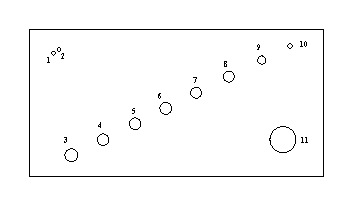
\includegraphics[width=0.75\linewidth]{pictures/acrylblock.pdf}
    \caption{Schematischer Querschnitt des Acrylblockes \cite{us2}.}
    \label{fig:acrylblock}
\end{figure}

Weiterhin soll das Auslösevermögen und die Dämpfung der Sonden bei verschiedenen Frequenzen untersucht werden.
Dafür wird eine A-Scan Messung bei den Fehlstellen 1 und 2 in \autoref{fig:acrylblock} gemacht.
Es wird eine 1 und \qty{2}{\MHz} Sonde untersucht. 

Schließlich soll mithilfe der Sonden noch in einem Brustmodell zwei Kugeln, die jeweils aus anderen Materialien bestehen, analysiert werden.
Dafür werden sie zunächst per Abtasten gefunden und dann mithilfe der Sonden analysiert.
Eine Kugel simuliert eine Zyste, die andere (festere) Kugel einen Tumor.